\section{A Brief Introduction to a JFET Transistor}
\label{lab_jfet}

%\makelabheader %(Space for student name, etc., defined in master.tex)

\bigskip

\begin{enumerate}[wide]

\item Build the circuit drawn below, which includes a 2N5457 transistor.  This is a new type of transistor called a ``Junction Field Effect Transistor,'' or JFET, and you've never seen anything like it before.  The three leads of this kind of transistor have different names than the BJT transistors you have seen so far.  The ``drain'' is analogous to the BJT's collector, the ``source'' is analogous to the emitter, and the ``gate'' is analogous to the base.  \textit{Notice that the 2N5457 pins are numbered differently from the previous transistor you used (the 2N3904), so be careful hooking it up!}  Measure the current through the source as you vary the gate voltage from 0 to $-2$ volts.  Make a rough plot of $I_S$ vs. $V_G$.
\begin{center}
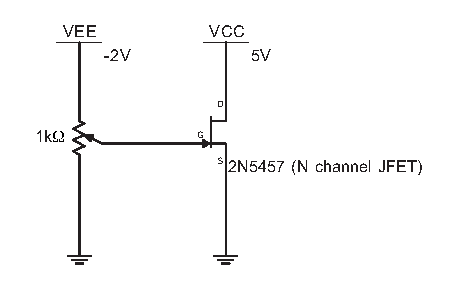
\includegraphics{jfet/JFET_test_circuit.eps}
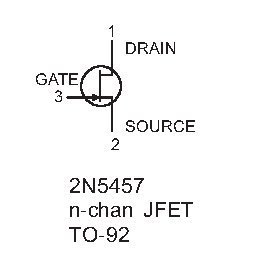
\includegraphics{appendices/pinouts/2N5457_pinout.eps}
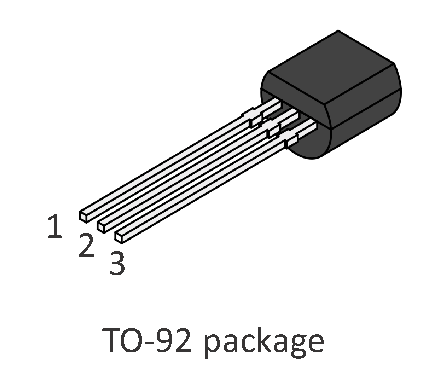
\includegraphics[width=1.3in]{appendices/pinouts/TO-92_package_pinout.eps}
\end{center}

\item Adjust the potentiometer so that the gate voltage is about $-0.5$ volts, and note the drain current.  Without changing the potentiometer adjustment, move your DMM to measure the current in the gate.  What's the ratio of $I_S/I_G$? \label{part_ratio_is_ig}

\item If you adjust $V_G$ to increase the magnitude of the current $I_G$, would that \textit{increase} or \textit{decrease} the current $I_S$?  Is the ratio $I_S/I_G$ a constant?

\item In previous labs, we learned two basic rules for analyzing BJT circuits: $V_E=V_B - 0.7$~volts, and $I_C/I_B=h_{FE}$ (a constant).   Does either of these two rules appear to hold true for the corresponding leads of this JFET transistor?  

\item Given your answer to part~\ref{part_ratio_is_ig}, what would be the advantage of using a transistor like this in an amplifier circuit?

\end{enumerate}








